%------------------------------------------------------------------------------
% CV in Latex
% Author : Charles Rambo
% Based off of: https://github.com/sb2nov/resume and Jake's Resume on Overleaf
% Most recently updated version may be found at https://github.com/fizixmastr 
% License : MIT
%------------------------------------------------------------------------------

\documentclass[A4,11pt]{article}
%\documentclass[letterpaper,14pt]{article} %For use in US
\usepackage{latexsym}
\usepackage[empty]{fullpage}
\usepackage{titlesec}
\usepackage{marvosym}
\usepackage[usenames,dvipsnames]{color}
\usepackage{verbatim}
\usepackage{enumitem}
\usepackage[hidelinks]{hyperref}
\usepackage[english]{babel}
\usepackage{tabularx}
\usepackage{tikz}
\usepackage[super]{nth}
\input{glyphtounicode}

\begin{comment}
I am by no means a professional when it comes to the CV's/resumes, I have
received various trainings on how to write a CV and resume from my high 
school, as well as the Austin College and University of Eastern Finland's
career counseling departments. As I intend to share my CV as a template, I 
feel that it is my responsibility to provide explanations of my work.
\end{comment}


%-----FONT OPTIONS-------------------------------------------------------------
\begin{comment}
The font of the document will impact not just how readable it is, but how it is
perceived. In the "The Craft of Scientific Writing" by Michael Alley, shares a
common fonts for publication as well as their use. I have chosen to use
Palatino for its legibility, some others are given below. There is far too much
about typography to discus here. Note: serif fonts have short projecting
strokes, sans-serif fonts are sans (without) these strokes.
\end{comment}


% serif
 \usepackage{palatino}
% \usepackage{times} %This is the default as well
% \usepackage{charter}

% sans-serif
% \usepackage{helvet}
% \usepackage[sfdefault]{noto-sans}
% \usepackage[default]{sourcesanspro}

%-----PAGE SETUP---------------------------------------------------------------

% Adjust margins
\addtolength{\oddsidemargin}{-1cm}
\addtolength{\evensidemargin}{-1cm}
\addtolength{\textwidth}{2cm}
\addtolength{\topmargin}{-1cm}
\addtolength{\textheight}{2cm}

% Margins for US Letter size
%\addtolength{\oddsidemargin}{-0.5in}
%\addtolength{\evensidemargin}{-0.5in}
%\addtolength{\textwidth}{1in}
%\addtolength{\topmargin}{-.5in}
%\addtolength{\textheight}{1.0in}

\urlstyle{same}

\raggedbottom
\raggedright
\setlength{\tabcolsep}{0cm}

% Sections formatting
\titleformat{\section}{
  \vspace{-4pt}\scshape\raggedright\large
}{}{0em}{}[\color{black}\titlerule \vspace{-5pt}]

% Ensure that .pdf is machine readable/ATS parsable
\pdfgentounicode=1

%-----CUSTOM COMMANDS FOR FORMATTING SECTIONS----------------------------------
\newcommand{\CVItem}[1]{
  \item\small{
    {#1 \vspace{-2pt}}
  }
}

\newcommand{\CVSubheading}[4]{
  \vspace{-2pt}\item
    \begin{tabular*}{0.97\textwidth}[t]{l@{\extracolsep{\fill}}r}
      \textbf{#1} & #2 \\
      \small#3 & \small #4 \\
    \end{tabular*}\vspace{-7pt}
}

\newcommand{\CVSubSubheading}[2]{
    \item
    \begin{tabular*}{0.97\textwidth}{l@{\extracolsep{\fill}}r}
      \text{\small#1} & \text{\small #2} \\
    \end{tabular*}\vspace{-7pt}
}

\newcommand{\CVSubItem}[1]{\CVItem{#1}\vspace{-4pt}}

\renewcommand\labelitemii{$\vcenter{\hbox{\tiny$\bullet$}}$}

\newcommand{\CVSubHeadingListStart}{\begin{itemize}[leftmargin=0.5cm, label={}]}
% \newcommand{\resumeSubHeadingListStart}{\begin{itemize}[leftmargin=0.15in, label={}]} % Uncomment for US
\newcommand{\CVSubHeadingListEnd}{\end{itemize}}
\newcommand{\CVItemListStart}{\begin{itemize}}
\newcommand{\CVItemListEnd}{\end{itemize}\vspace{-5pt}}

%------------------------------------------------------------------------------
% CV STARTS HERE  %
%------------------------------------------------------------------------------
\begin{document}

%-----HEADING------------------------------------------------------------------

\begin{minipage}[c]{0.05\textwidth}
  \-\
\end{minipage}
\begin{minipage}[c]{0.3\textwidth}
  \begin{tikzpicture}
    \clip (-1.8,-1.5) circle (2.cm);
    % \node at (-1.9,-2.) {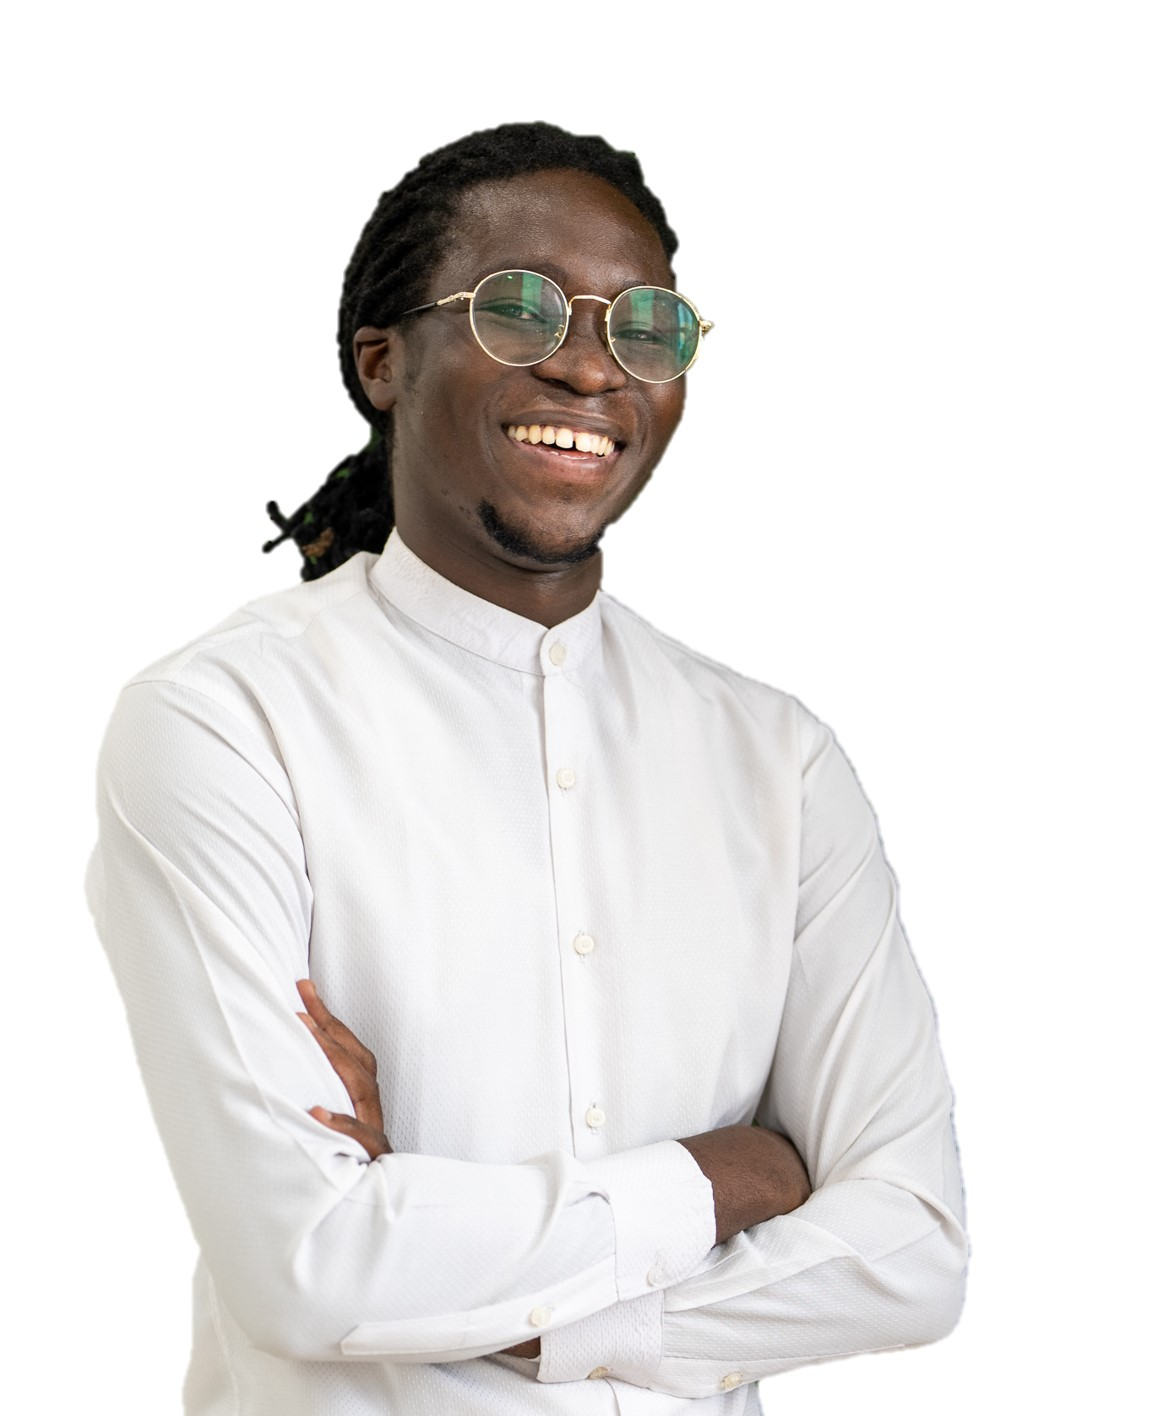
\includegraphics[width = 5.5cm]{HeadShot_Cedric_MANOUAN}};
    \node at (-2.3,-2.3) {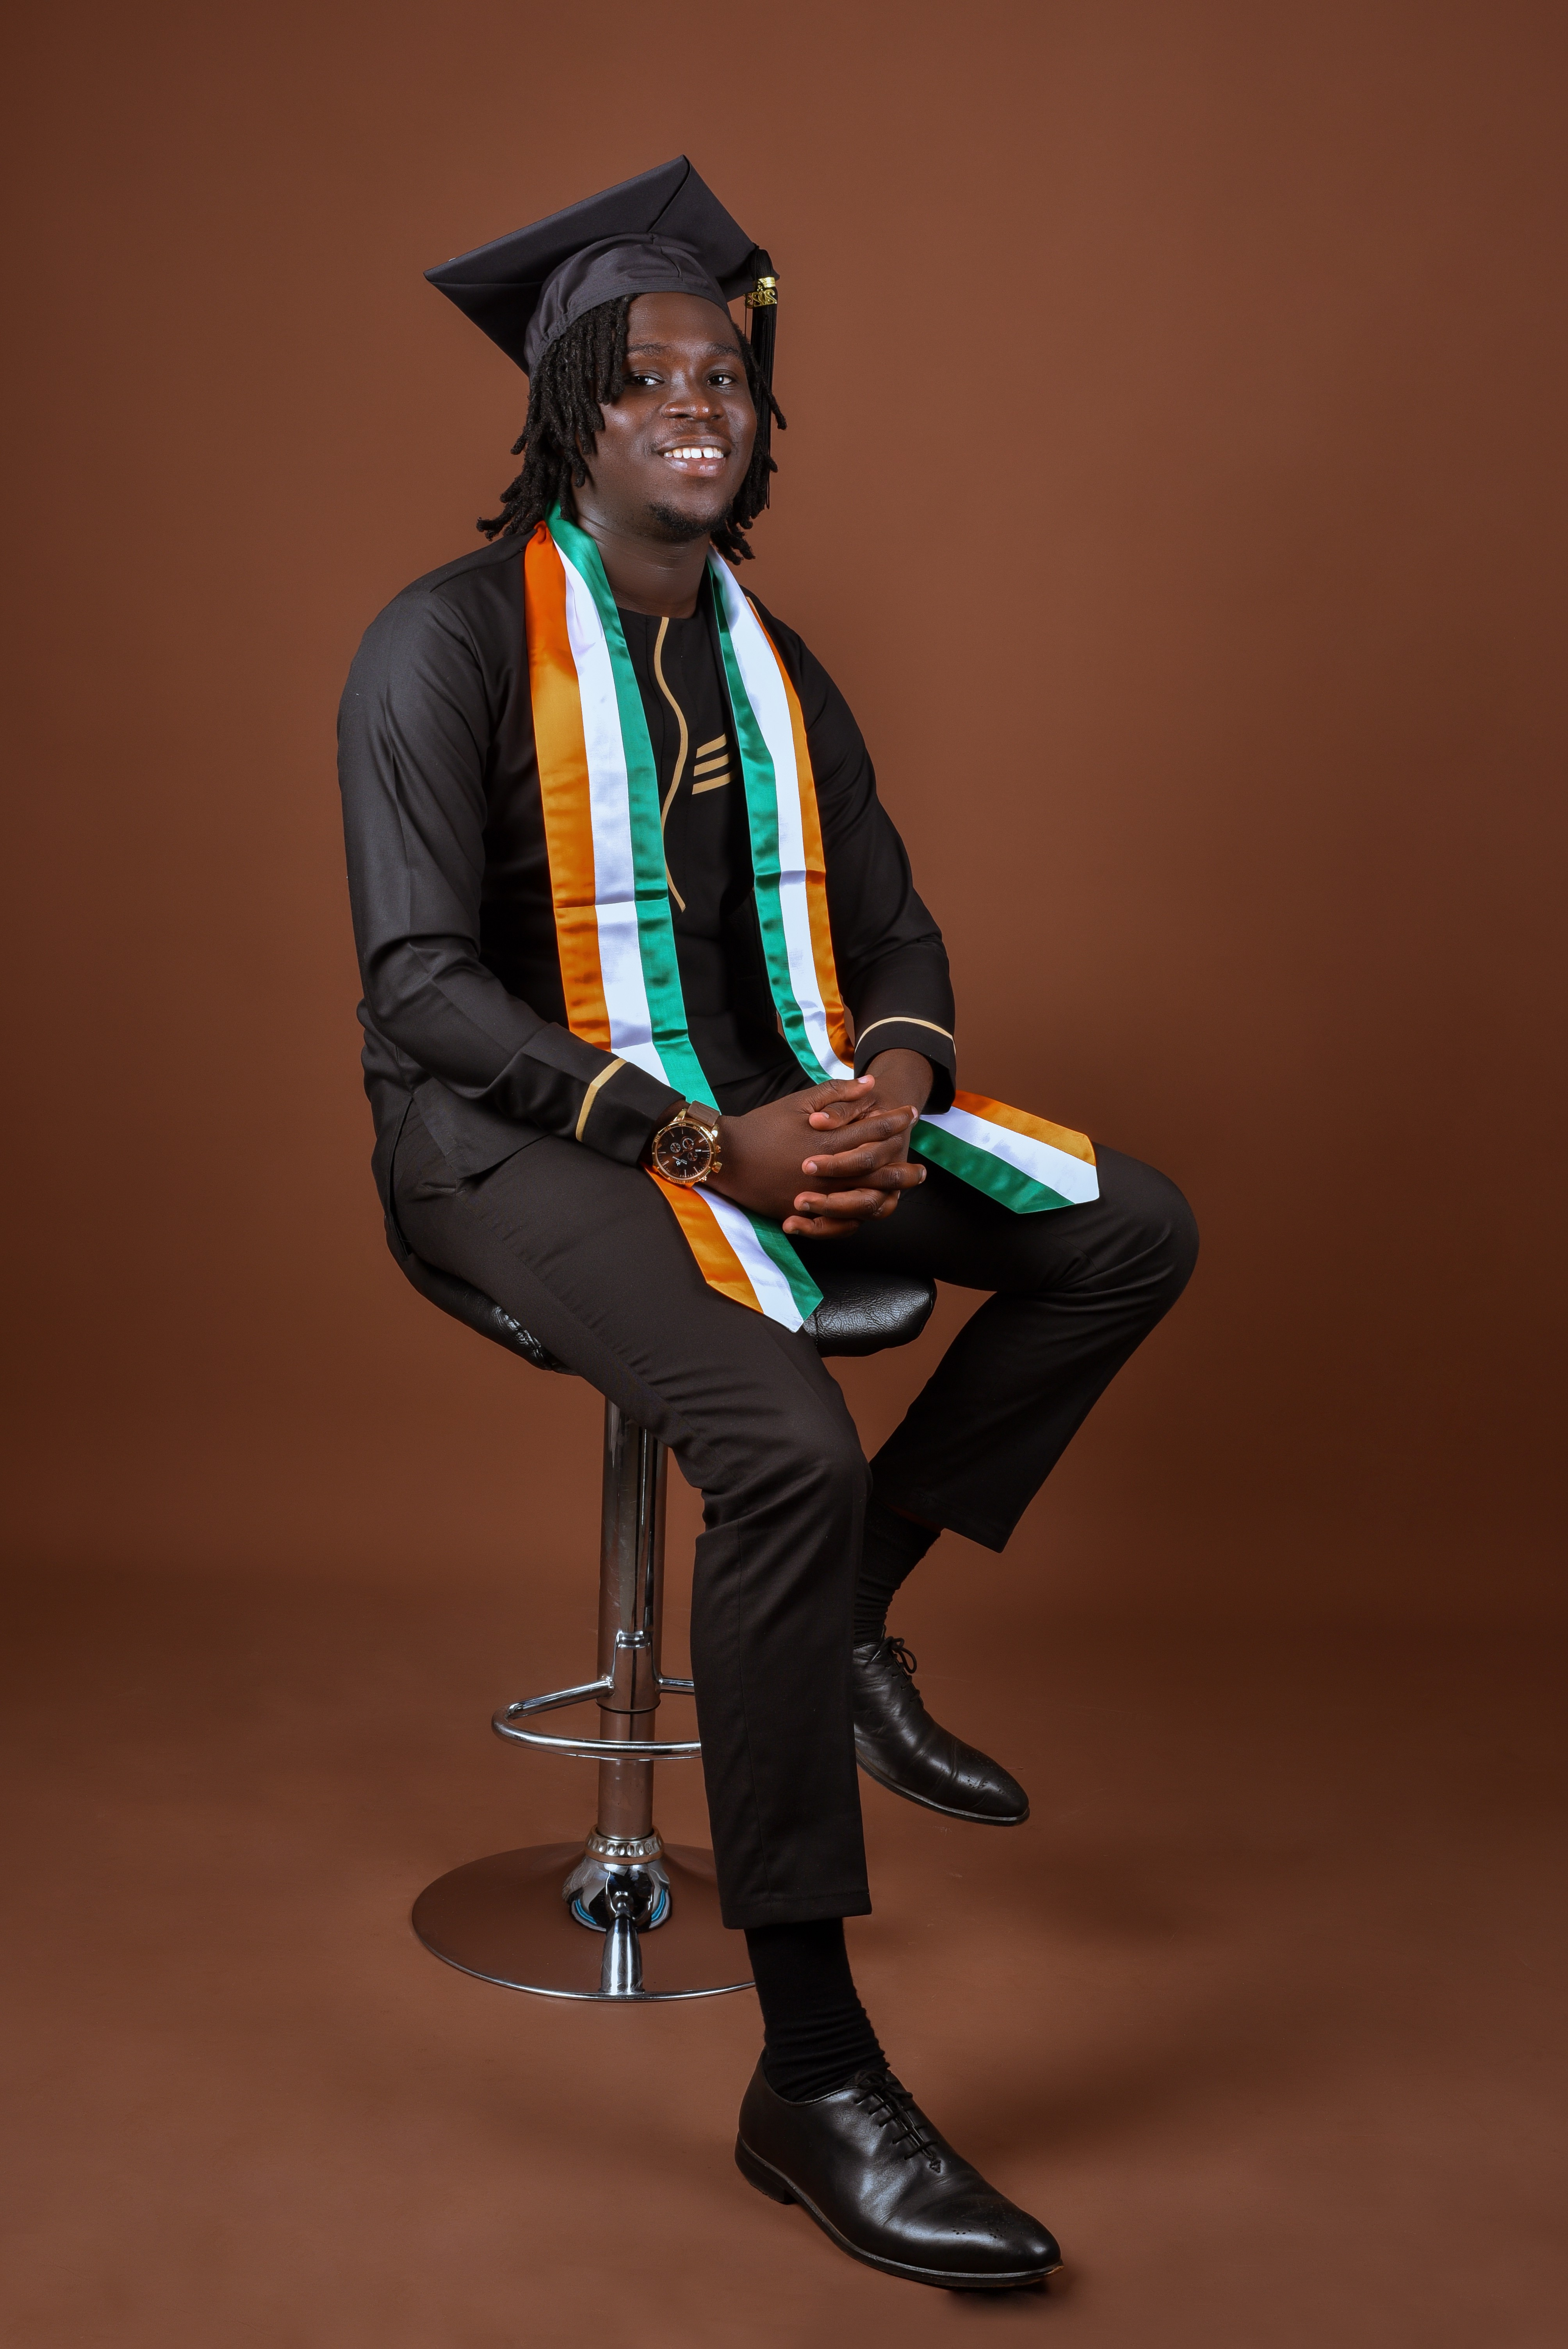
\includegraphics[width = 4.5cm]{SSP_3357}};

  \end{tikzpicture}
  \hfill\vline\hfill
\end{minipage}
\begin{minipage}[c]{0.6\textwidth}
\textbf{\Huge \scshape{Cédric P.-E. MANOUAN}}\\\vspace{1pt}
\textbf{Deep Learning Engineer}\\
%{\textbf{Phylosophy}:
%\begin{quote}
%  \small ``The world is being built on code. It is not bricks and mortars anymore.``
%\end{quote}
%\hfill(\emph{\textbf{\small Joshua MWANIKI}})
%}

%\scshape sets small capital letters, remove if desired
\small{\textbf{Adresse : }Kigali, Rwanda} \\
\small{\textbf{Contact : }+250 (0) 791 591 607} \\
%\small{\textbf{Birthdate : }15 February 1999} \\
\href{mailto:cmanouan@alumni.cmu.edu}{\textbf{Email:} cmanouan@alumni.cmu.edu}\\
%Be sure to use a professional *personal* email address
\href{https://www.linkedin.com/in/cpem/}{\textbf{Linkedin:} Cédric pascal-emmanuel MANOUAN} \\
%you should adjust you linked in profile name to be professional and recognizable
\href{https://github.com/dric2018/}{\textbf{Github:} dric2018}
\end{minipage}

% Without picture
%\begin{center}
%  \textbf{\LARGE \scshape Cedric P.-E. MANOUAN} \\ \vspace{1pt} %\scshape sets small capital letters, remove if desired
%  \small{\textbf{Contact : }+250 (0) 791 591 607} $|$
%  \href{mailto:cmanouan@andrew.cmu.edu}{\textbf{Email:} cmanouan@andrew.cmu.edu} $|$ \\
  % Be sure to use a professional *personal* email address
%  \href{https://www.linkedin.com/in/c%C3%A9dric-pascal-emmanuel-manouan-ba9ba1181/} {\textbf{Linkedin:} Cédric pascal-emmanuel MANOUAN} $|$ 
  % you should adjust you linked in profile name to be professional and recognizable
%  \href{https://github.com/dric2018/}{\textbf{Github:} dric2018}\\

%\end{center}

%-----Summary----------------------------------------------------------------
%\section{Résumé}
%Développeur de logiciels/machine learning spécialisé dans l'apprentissage profond depuis plus de 3 ans. Travailleur acharné, capable de travailler de façon autonome avec un bon esprit d'équipe. Expérience dans des projets d'apprentissage automatique : je peux travailler de la préparation des données à la définition et à l'optimisation des modèles ; c'était presque tout mon travail à Zindi.
%Capacité à évoluer dans un environnement collaboratif (même à distance) tout en maintenant le m\^eme niveau d'efficacité.


%-----EDUCATION----------------------------------------------------------------
\section{Education}
\CVSubHeadingListStart
\CVSubheading
{{Master Scientifique $|$ \emph{\small{Technologies de l'Information}}}}{Ao\^ut 2021 -- Mai 2023}
{Carnegie Mellon University}{Kigali, Rwanda}
\CVSubheading
{{Master Scientifique (Bac+4) $|$ \emph{\small{Systemes informatiques et Génie logiciel}}}}{Octobre 2019 -- Mars 2020}
{Ecole Supérieure Africaine des TIC (ESATIC) }{Abidjan, Côte d'Ivoire}
\CVSubheading
{Licence Générale $|$ \emph{\small{Systèmes, Réeaux Informaiques et Télécommunications}}}{Octobre 2016 -- Septembre 2019}
{Ecole Supérieure Africaine des TIC (ESATIC) - \href{https://drive.google.com/file/d/1AHcLovrqVw6Awh7r_sUYj2X1VdPfAZGq/view?usp=sharing}{Clicker pour voir mon attestation}}{Abidjan, Côte d'Ivoire}
\CVSubHeadingListEnd

%-----WORK EXPERIENCE----------------------------------------------------------

\section{Expérience professionnelle}
\CVSubHeadingListStart

\CVSubheading
{Stagiaire en ingénieurie informatique/Science des données}{Mai 2021 -- Juillet 2021}
{Zindi}{Remote (Entreprise basée en Afrique du Sud)}
\CVItemListStart
\CVItem{Préparation des compétitions de science de données}
\CVItemListEnd

\CVSubheading
{Stagiaire en développement informatique (Projet de fin de cycle)}{Avril 2019 -- Juin 2019}
{Projet de Solutions Numériques pour le Désenclavement des Zones Rurales et l'E-Agriculture\\(PSNDEA)}{Abidjan, Côte d'Ivoire}

\CVItemListStart
\CVItem{Conception d'un Système IoT pour la collecte de données en provenance d'un champ de manioc}
\CVItem{Développement d'une API REST CRUD basée sur un serveur NodeJS et une base de donnée MySQL pour le stockage des données recueillies par les capteurs}
\CVItem{Développement d'un modèle de regression pour la prediction du rendement de la plantation utilisant les données en temps réel et celles précédemment collectées}
\CVItem{Déploiement du modèle d'apprentissage automatique sur un appareil embarqué (Raspbery Pi 3) via l'API Tensorflow JS}
\CVItemListEnd
\CVSubHeadingListEnd

%-----SKILLS-------------------------------------------------------------------
\section{Compétences}
\begin{itemize}[leftmargin=0.5cm, label={}]
  \small{\item{
\textbf{Langues}{: Français (Langue maternelle), Anglais (Bilingue, couramment parlé)} \\
\textbf{Programmation}{:
          \begin{itemize}
\item Python \\
                  \begin{itemize}
\item \textbf{Calcul scientifique}: NumPy
\item \textbf{Visualisation de données}: Matplotlib, Seaborn
\item \textbf{Manipulation de données}: Pandas
\item \textbf{Machine learning}: Scikit-learn, Lightgbm/Xgboost (\textbf{Bonnes notions})
\item \textbf{Deep learning}: Pytorch, Tensorflow/Keras 

                  \end{itemize}
\item C++ 
\item Bash/automatisation de tâches (\textbf{Bonnes notions})

\item JavaScript (\textbf{Bonnes notions})
                  \begin{itemize}
\item Développement backend avec NodeJS
                  \end{itemize}
\item Développement HTML/CSS/Développement web  

          \end{itemize}

        }
\textbf{Conception de documents}{: Microsoft Office, LaTeX, Markdown} \\
\textbf{Cloud computing / Gestion de code / DevOps}{: Git, Docker, Amazon Web Services (EC2/ECS)} \\
\textbf{Systèmes d'exploitation}{: Ubuntu, Mac OS} \\
        }}
\end{itemize}

%-----PROJECTS AND RESEARCH----------------------------------------------------
\section{Projets}
\CVSubHeadingListStart
\CVSubheading
{{Competition - Science des données - Classification d'Images} $|$ \emph{\small{ZINDI}}}{Automne 2020}
{ Compétition éducative de développement d'un algorithme machine learning pour la classification \\
d'images médicales de patients attteints de tuberculose ou non.\\
\textbf{Position} : 7e/104, \textbf{\href{https://zindi.africa/competitions/runmila-ai-institute-minohealth-ai-labs-tuberculosis-classification-via-x-rays-challenge/leaderboard}{ Voir team DataLabCI sur le leaderboard}} \\
\textbf{Lien du projet} : \href{https://github.com/dric2018/ZindiTuberculosisClassification}{Tuberculosis X-Rays classification}
}{}

\CVSubheading
{{Competition - Science des données - Classification d'Audios} $|$ \emph{\small{ZINDI}}}{Automne 2020}
{ Contribution au développement d'un algorithme de machine learning pour la classification \\
de données audio en anglais et Luganda (Uganda) \\
\textbf{Position} : 7e/255, \textbf{\href{https://zindi.africa/competitions/giz-nlp-agricultural-keyword-spotter/leaderboard}{Voir team wakanda sur leaderboard}} \\
\textbf{Lien du projet} : \href{https://github.com/NazarioR9/GIZ-NLP-Agricultural-Keyword-Spotter}{GIZ-NLP-Agricultural-Keyword-Spotter}
}{}

\CVSubheading
{{Hackathon - Science des données - Classification d'Images} $|$ \emph{\small{ZINDI}}}{Automne 2020}
{Contribution au développement d'un algorithme d'apprentissage automatique pour la classification \\
binaire d'images de personnes portant un masque ou non.\\
\textbf{Position} : 3e, \textbf{ \href{https://zindi.africa/competitions/spot-the-mask-challenge}{Voir team TheCIA sur leadernoard}} \\
\textbf{Lien du projet} : \href{https://github.com/NazarioR9/Spot-the-Mask-challenge-3rd-Place}{Face mask classification}
}{}

\CVSubheading
{{[Hackathon] 1er prix Niveau 2 (48h) - Reconnaissance d'images} $|$ \emph{\small{ESATIC}}}{Mai 2018}
{Contribution au développement d'un algorithme de deep learning \\
pour la reconnaissance de billets de banque
}{}

\CVSubheading
{{[Hackathon] 1er prix Niveau 1 (24h) - Cryptographie} $|$ \emph{\small{ESATIC}}}{Mai 2017}
{Conribution à l'analyse et au développement d'un algorithme de cryptage via reverse engineering.

}{}

\CVSubHeadingListEnd

%-----CONFERENCES AND PRESENTATIONS--------------------------------------------

%-----HONORS AND AWARDS--------------------------------------------------------
\section{Reconnaissances}
\CVSubHeadingListStart
\CVSubheading
{Brourse d'études MasterCard Foundation}{2021 -- 2023}
{Programme de bourses destinées à soutenir les étudiants ayant démontré des compétences de leadership}{}

\CVSubHeadingListEnd

%-----TEACHING EXPERIENCE------------------------------------------------------

%\section{Teaching Experience}
%\CVSubHeadingListStart
%    \CVSubheading
%      {What}{When}
%      {School}{Where}
%\CVSubheading
%{High School Physics (11 Weeks Teaching/Observing)}{Fall 2017}
%{Denison High School}{Denison, TX}
%\CVSubheading
%{High School Calculus (11 Weeks Teaching/Observing)}{Fall 2017}
%{Denison High School}{Denison, TX}
%\CVSubheading
%{High School Geometry (9 Weeks Teaching/Observing)}{Spring 2016}
%{Sherman High School}{Sherman, TX}
%\CVSubHeadingListEnd

%-----COMMUNITY INVOLVEMENT----------------------------------------------------
\section{Engagement communautaire}
\CVSubHeadingListStart
%    \CVSubheading %Example
%      {What you did}{When you worked there}
%      {Who you worked for}{Where they are located}

\CVSubheading
{Club de Science des données }{Decembre 2021 -- Aujourd'hui}
{Lead et coordonnateur}{Rwanda, Kigali, CMU-Africa}

\CVSubheading
{Data Science Côte D'Ivoire}{2020 -- Aujourd'hui}
{Mentorat pour les étudiants et autres passionnés de science des données}{Côte d'Ivoire, remote}

\CVSubheading
{Zindi University ambassador}{Juin 2020 -- Juillet 2021}
{}{Côte d'Ivoire, remote}
\CVItemListStart
\CVItem{Participation à plusieurs compétitions (nom d'utilisateur : \href{https://zindi.africa/users/I_am_Zeus_AI/competitions}{\textbf{I\_am\_Zeus\_AI}})}%, Top 100 among zindi data scientists}
\CVItem{ Co-lead du groupe de développement (plateforme, amélioarations et nouvelles idées)}
\CVItem{Recrutement de participants pour le hackathon universitaire UMOJAHACK 2021 (plus de 15 nouveaux)}
\CVItemListEnd

\CVSubheading
{Membre fondateur du club Objets connectés et Intelligence Artificielle}{2019}
{ESATIC}{Abidjan, Côte d'Ivoire}
\CVSubHeadingListEnd

\section{Autres Qualités}
\CVItemListStart
\CVItem{Motivateur \& Leader}
\CVItem{Preneur d'initiative}
\CVItem{Résolveur de problème}
\CVItemListEnd
%------------------------------------------------------------------------------
\end{document}